\begin{frame}{Convolution Encode}

\begin{center}
\begin{minipage}{.45\textwidth}
\begin{center}
\begin{tabular}{c c c c}
  \visible<1-> {state&input&output&next state\\ \hline}
   \visible<2-> { 00 & 1 & 11 & 10 \\  } \visible<3-> { 10 & 0 & 10 & 01 \\  } \visible<4-> { 01 & 1 & 00 & 10 \\ \hline } \visible<5-> { 10 & 0 & 10 & 01 \\ } \visible<6-> { 01 & 0 & 11 & 00 \\ }
\end{tabular}
\end{center}
\end{minipage}
\hfill
\begin{minipage}{.45\textwidth}
\begin{center}
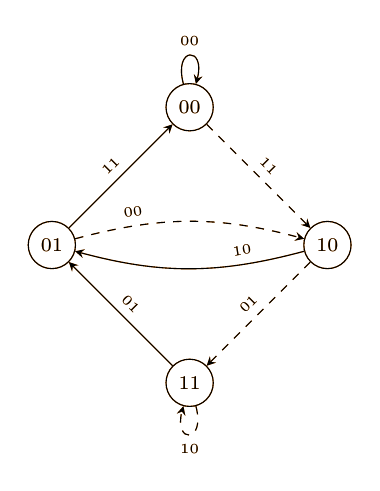
\begin{tikzpicture}[scale=.70, >=stealth, font=\tiny]
\tikzstyle{state} = [draw, circle, inner sep=1mm, minimum size=6mm, font=\scriptsize]
 \alt<2> {\node[state, orange] (state0) at (0,2.5) {00};}{\node[state] (state0) at (0,2.5) {00};}; \alt<3,5> {\node[state, orange] (state2) at (2.5,1.53075794227797e-16) {10};}{\node[state] (state2) at (2.5,1.53075794227797e-16) {10};}; \alt<0> {\node[state, orange] (state3) at (3.06151588455594e-16,-2.5) {11};}{\node[state] (state3) at (3.06151588455594e-16,-2.5) {11};}; \alt<4,6> {\node[state, orange] (state1) at (-2.5,-4.59227382683391e-16) {01};}{\node[state] (state1) at (-2.5,-4.59227382683391e-16) {01};}; \alt<0> {\draw[->, orange] (state0) to [looseness=8,out=105,in=75] node [sloped, above] {00} (state0) ;}{\draw[->] (state0) to [looseness=8,out=105,in=75] node [sloped, above] {00} (state0) ;}; \alt<2> {\draw[->, dashed, orange] (state0) to  node [sloped, above] {11} (state2) ;}{\draw[->, dashed] (state0) to  node [sloped, above] {11} (state2) ;}; \alt<6> {\draw[->, orange] (state1) to  node [sloped, above] {11} (state0) ;}{\draw[->] (state1) to  node [sloped, above] {11} (state0) ;}; \alt<4> {\draw[->, dashed, orange] (state1) to [bend left=15] node [sloped, above,near start] {00} (state2) ;}{\draw[->, dashed] (state1) to [bend left=15] node [sloped, above,near start] {00} (state2) ;}; \alt<3,5> {\draw[->, orange] (state2) to [bend left=15] node [sloped, above,near start] {10} (state1) ;}{\draw[->] (state2) to [bend left=15] node [sloped, above,near start] {10} (state1) ;}; \alt<0> {\draw[->, dashed, orange] (state2) to  node [sloped, above] {01} (state3) ;}{\draw[->, dashed] (state2) to  node [sloped, above] {01} (state3) ;}; \alt<0> {\draw[->, orange] (state3) to  node [sloped, above] {01} (state1) ;}{\draw[->] (state3) to  node [sloped, above] {01} (state1) ;}; \alt<0> {\draw[->, dashed, orange] (state3) to [looseness=8,out=285,in=255] node [sloped, below] {10} (state3) ;}{\draw[->, dashed] (state3) to [looseness=8,out=285,in=255] node [sloped, below] {10} (state3) ;};
\end{tikzpicture}
\end{center}
\end{minipage}
\end{center}

\end{frame}

\begin{frame}{state color matrix}

2

4,6

3,5

\end{frame}
